\documentclass[final,letterpaper]{article}

\usepackage{url}
\usepackage{graphicx}
\usepackage[hidelinks]{hyperref}
\usepackage{pdfpages}
\usepackage{geometry}
\usepackage{caption}
%\usepackage[caption=false]{subcaption}


\newcommand{\baposter}{\texttt{baposter}}
\newcommand{\posterbox}{\texttt{posterbox}}

\title{The baposter latex poster style}
\author{Brian Amberg and Reinhold Kainhofer and Stefan McKinnon H{\o}j-Edwards }

\begin{document}
\maketitle
\begin{abstract}
This is still only a very rough documentation, but it should be better than no
documentation. If anything is unclear, please post a request (preferably with a
patch) at the bugtracker.
This document is for \baposter{} v. 2.1.
\end{abstract}

\section{Introduction}
\baposter{} is a LaTeX template to efficently design pretty posters for
scientific conferences. Posters are composited of blocks with headings, which
can be positioned easily on the page, using absolute or relative positioning. A
number of predefined styles can be composed to generate new color schemes and
ornaments.

\section{Usage}
Refer to the included example posters for the overall structure.
Here, we will document the different keys together with small examples.
The main environment for the poster is the \texttt{poster} environment. It has the following structure
\begin{verbatim}
\begin{document}
\begin{poster}{
  key=value options
  }
  {
    Left / top logo
  }
  {
    Poster Title
  }
  {
    Poster Authors
  }
  {
    Right logo
  }

  Definition of the boxes
\end{poster}
\end{document}
\end{verbatim}

It must be immediately inside the \texttt{document}-environment, or there will be blank pages.

The top portion of a poster can be setup to one of three settings as shown in figure \ref{structure}. \texttt{logosetup=leftright} is default.
\begin{figure}[h]
    \centering
    %\begin{subfigure}[b]{0.3\textwidth}
        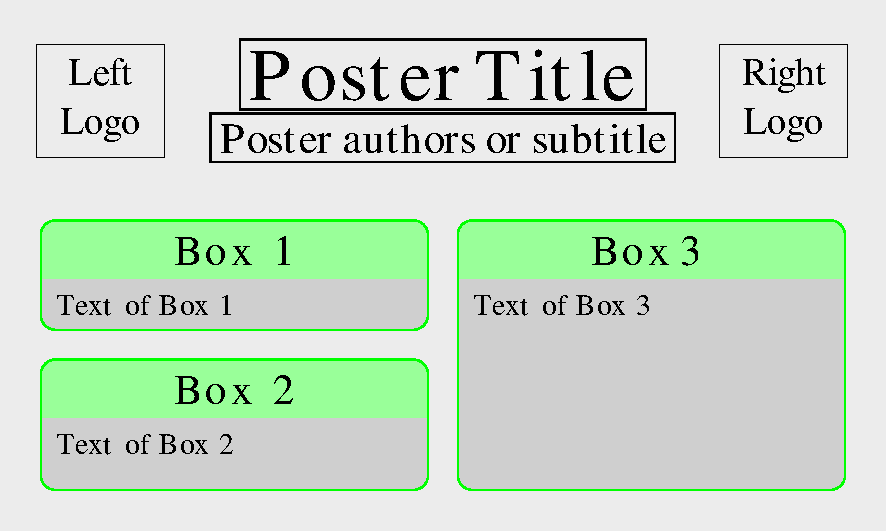
\includegraphics[width=0.3\textwidth]{docs-structure-leftright}
    %    \caption{\texttt{logosetup=leftright}}
    %    \label{structure:leftright}
    %\end{subfigure}
    ~
    %\begin{subfigure}[b]{0.3\textwidth}
        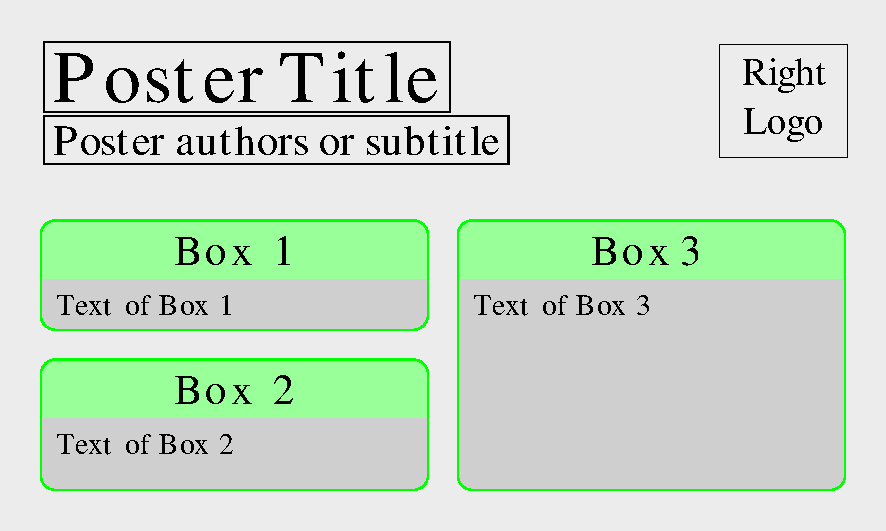
\includegraphics[width=0.3\textwidth]{docs-structure-right}
    %    \caption{\texttt{logosetup=right}}
    %    \label{structure:right}
    %\end{subfigure}
    ~
    %\begin{subfigure}[b]{0.3\textwidth}
        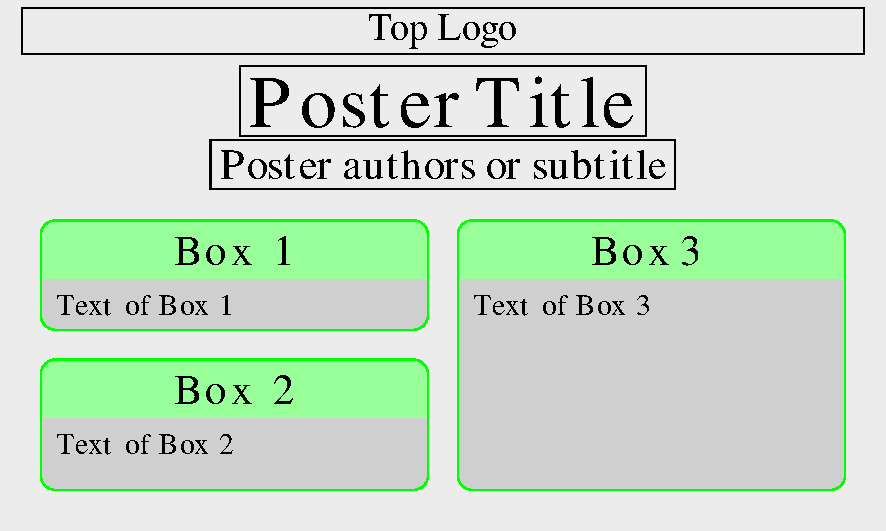
\includegraphics[width=0.3\textwidth]{docs-structure-topbar}
    %    \caption{\texttt{logosetup=topbar}}
    %    \label{structure:topbar}
    %\end{subfigure}
    \caption{3 structures of header of poster using \texttt{logosetup} option, from left to right, \texttt{leftright}, \texttt{right} and \texttt{topbar}.}
    \label{structure}
\end{figure}


Additionally, you can pass some options for page size selection directly to the class file.
\begin{verbatim}
\documentclass[class options]{baposter}
\end{verbatim}


\subsection{The posterbox environment}
After defining the paper size in class options, logos and poster appearences, you will need to place contents on your poster.
This is done with the \posterbox{}\footnote{Replacing the now deprecated \texttt{headerbox}.} environment:
\begin{verbatim}
 \begin{posterbox}[name=conclusion,column=0,row=0]{Conclusion}
  My conclusions...
 \end{posterbox}
\end{verbatim}
This will produce a small box, at the top of the first column with a small header (``Conclusion'').

Positioning and sizing of a \posterbox{} can be done both absolute and relative to other boxes.
By using \texttt{[column=0,row=0.2]} the box is placed in the \emph{first} column at 20\% of the columns height.
Naturally, by specifying \texttt{[row=0]}, the box is placed at the top of the column.

The vertical position can be specified relative to other boxes by using the \texttt{above}, \texttt{aligned} and \texttt{below} options, 
e.g.\ a \posterbox{} that appears below the conclusion box, but in another column could be declared as
\begin{verbatim}
  \begin{posterbox}[name=method,column=1,below=conclusion]{Methods for this}
    I placed a cat in a box...
  \end{posterbox}
\end{verbatim}
For this to work, a referenced \posterbox{} \emph{must} be declared above in the \LaTeX  source text.

Finally, the size can be set by using the \texttt{bottomaligned}, \texttt{height} and \texttt{span} options.
The first two specifies the height, as in the bottom of a \posterbox{} will flow down to the bottom of the referenced \posterbox{} and/or the height absolute set as a fraction of the column height,
and the last specifies how many columns the \posterbox{} should span.

\section{Options}

\subsection{Class options}
The class options are

\begin{description}
\item [landscape/portrait] Page Layout
\item [a0paper, a1paper, a2paper, a3paper, a4paper, archE] Predefined paper sizes
\item [paperwidth=length,paperheight=length] Width/Height of the paper. Do not use together with a0paper or other predefined paper sizes.
\item [margin=length] Page margin
\item [fontscale=real number] Scaling of the poster. The poster is typeset with
standard font sizes on a `fontscale times papersize' paper, and then scaled up
by 1/fontscale to the chosen paper size. This ensures good looking font sizes.
So if you need to fit more onto a poster, increase the fontscale option to get
smaller fonts. But be sure not to choose too small fonts, or your paper will be
awful. I find posters with small print a nuisance, and tend to spend more time
with well presented and concise content.
\item [showframe] Show a frame around the page, mainly useful for debugging.
\item [movebody] Moves text/poster body to the right (or left if negative),
\end{description}

\subsection{Poster Environment Options}

The available options for the poster environment are:
\begin{description}
  \item[grid=\{true,false\}]                Display a grid, which can be useful during the layout phase.
  \item[columns=4] Number of columns (default 4 in landscape and 3 in portrait format) (maximum number is 6).
  \item[colspacing=length]              Distance between the columns of the poster.
  \item[headerheight=length]            Height of the main poster header as a length (not of the headers of the text boxes). Default value is \verb+0.1\textheight+.
  \item[background=poster background type] Type of poster background. Possible values are
  \begin{enumerate}
    \item \verb+plain+: Plain background in one color (\verb+bgColorOne+)
    \item \verb+shadeLR+: Horizontal background gradient (from \verb+bgColorOne+ to \verb+bgColorTwo+)
    \item \verb+shadeTB+: Vertical background gradient (from \verb+bgColorOne+ to \verb+bgColorTwo+)
    \item \verb+user+: Use the command \verb|\background{...}| to define your own background.
    \item \verb+none+: No background at all.
  \end{enumerate}
  \begin{center}
    \setlength{\fboxsep}{0pt}

    \fbox{\includegraphics[width=0.21\textwidth,page=1]{docs-background}}
    \fbox{\includegraphics[width=0.21\textwidth,page=2]{docs-background}}
    \fbox{\includegraphics[width=0.21\textwidth,page=3]{docs-background}}
    \fbox{\includegraphics[width=0.21\textwidth,page=4]{docs-background}}
  \end{center}

  \item[bgColorOne=pgf color name]      First background color. For a plain, this color will be used. For a shaded background, this is the first color for the gradient.
  \item[bgColorTwo=pgf color name]      Second background color. This color will only be used for shaded backgrounds as the end color of the gradient.
  \item[logosetup=\{leftright, right, topbar\}]
                                        Selects a setup for the logos, see figure \ref{structure}.
  %\item[eyecatcher=\{yes,no\}]           Should an eye catcher be shown on the
  %                                       left of the title page. The eyecatcher itself is defined in the second
  %                                       argument of the poster environment.

\end{description}

\subsection{Posterbox Environment Options}

\begin{description}
  \item[name]                           Name the \posterbox{} for later refering. 
  \item[borderColor=pgf color name]     Color used for the borders of the poster boxes
  \item[headerColorOne=pgf color name]  First color of box header. Two colors can be used to define gradients.
  \item[headerColorTwo=pgf color name]  Second color of box header. Two colors can be used to define gradients.
  \item[textborder=border type]         Which kind of border should the lower part of the text boxes have. Possible values are:
  \begin{enumerate}
    \item none
    \item bars
    \item coils
    \item triangles
    \item rectangle
    \item rounded
    \item faded
  \end{enumerate}
\includegraphics[width=0.9\textwidth]{docs-boxshape}

  \item[headerborder=header border type] At which sides of the text box headers should we draw a border. Possible values are:
  \begin{enumerate}
    \item none
    \item closed
    \item open
  \end{enumerate}
\includegraphics[width=0.9\textwidth]{docs-headerborder}
  \item[headershape=header border shape] The type of ornament of the text box headers. Possible values are
  \begin{enumerate}
    \item rectangle
    \item small-rounded
    \item roundedright
    \item roundedleft
    \item rounded
  \end{enumerate}
\includegraphics[width=0.9\textwidth]{docs-headershape}
  \item[headershade=type of header shading] Which shading should be applied to the text box headers. Possible values are
  \begin{enumerate}
    \item plain
    \item shade-lr
    \item shade-tb
    \item shade-tb-inverse
  \end{enumerate}
  \item[boxshade] which kind of shading is applied to the text boxes. Possible values are
  \begin{enumerate}
    \item shade-lr
    \item shade-tb
    \item plain
    \item none
  \end{enumerate}
  \item[headerfont=font definition]      Commands inserted before a text box header is typeset.
  \item[headerFontColor=pgf color name]  Color that the header is typeset in.
  \item[linewidth=length] Width of the lines used when drawing the poster.
  
  \item[column=integer] Which column should the \posterbox{} be in. Counting starts at 0.
  \item[row=real number] At which fraction of the columns height should the top of the \posterbox{} be at?
  \item[above=\emph{name},below=\emph{name}] Positions a \posterbox{} above or below another \posterbox{}; the referenced \posterbox{} must be specified prior!
  \item[height=real number,bottomaligned=\emph{name}] Sets the height as a fraction of the column and/or aligns the bottom to that of another \posterbox{}.
  \item[span=integer] How many columns should the \posterbox{} span?
\end{description}

\section{Author and Licence}
The original author is Brian Amberg, and the class and documentation has been
greatly improved by Reinhold Kainhofer.
Further work was done by Stefan McKinnon H{\o}j-Edwards in 2013.
The class is distributed under the GPL.
The current version and documentation can be found at:
\begin{center}
\url{http://www.brian-amberg.de/uni/poster/}
\end{center}
\end{document}

